\subsection{Magnet Design}\label{cap:methoden_magnet_design}
Die Form des Magneten war abhängig von mehreren Faktoren. Einerseits musste der Magnet anhand der elektronischen Vorgaben angepasst werden, anderseits limitierte das Rad des Fitnesstrainers den Platz für den Magnet.



\begin{figure}[ht]
    \begin{center}
      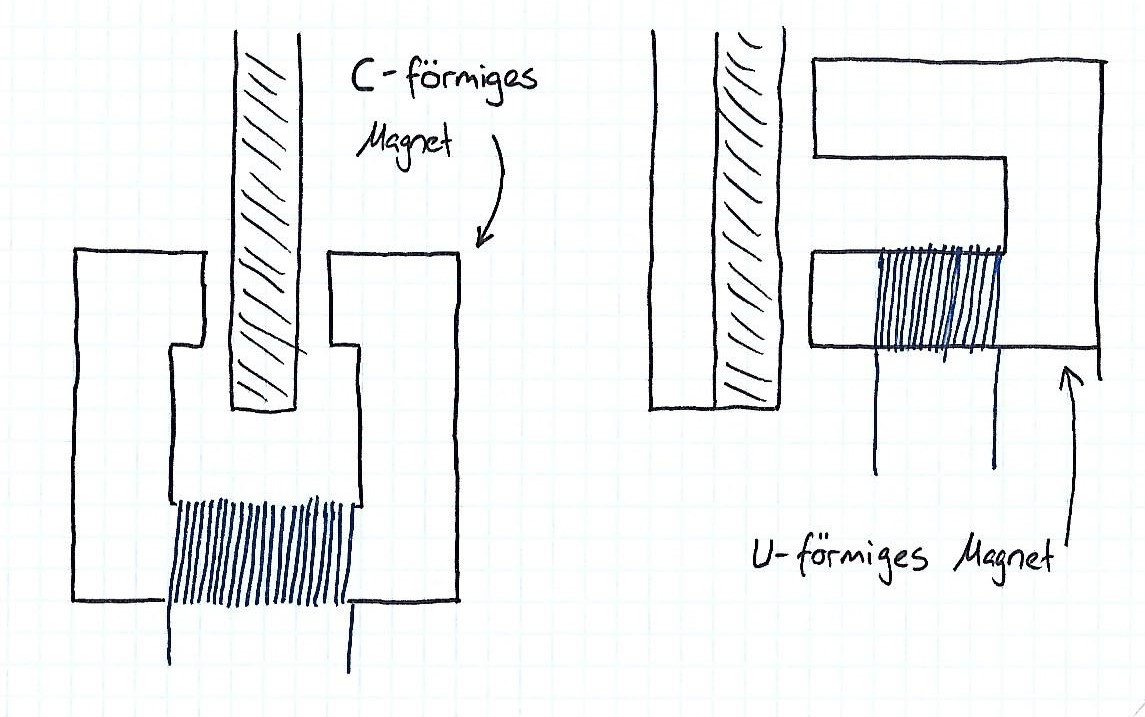
\includegraphics[width=12cm]{assets/images/magnet_uc}
    \end{center}
    \vspace{-3ex}
    \caption{U-förmiges und C-Förmiges Magnet}
    \label{fig:magnet_uc}
  \end{figure}

Im Normalfall besteht eine Magnetbremse aus einer Metall-Scheibe, welche eine gute Leitfähigkeit besitzt, und einem C-förmiger Magnet, welcher in der Öffnung die Scheibe platziert wird. Wenn der Platz ungenügend ist, kann eine zusätzliche eisenhaltige Scheibe hinzugefügt werden und der C-förmige Magnet durch einen U-förmigen Magnet ersetzt werden, wobei dieser nicht unten platziert wird, sondern seitlich der Scheibe (Siehe Abbildung \ref{fig:magnet_uc}). Dieser Aufbau erlaubt es, die zu bremsende Scheibe von der Seite an zu bremsen, anstatt von unten. Der Nachteil ist der Energieverlust zwischen den Luftspalten, welcher sich fast verdoppelt. 
\newpara
Da das Rad des Fitnesstrainers zu breit ist und daher den Platz für ein C-förmiger Magnet zu eng ist, wurde für ein U-förmiges Magnet entschieden. Im Anhang können die Pläne für die Eisen- und Aluminium-Platte und für das Magnet gefunden werden. Diese Pläne wurden in der CAD-Software \textit{Fusion 360} von Autodesk erstellt.
\newpara
Der Magnet wurde anhand der von W.R. Smythe geschriebenen Arbeit \textit{Eddy Current on a Rotating Disk}(\cite{current_on_a_rotating_disk}) erstellt. Diese Formel wurde von Empfehlung einer externen Person verwendet, da diese Person mit dieser Formel gearbeitet hatte. Von Smythes Arbeit wurde die Formel 22 für die Berechnung des Magneten verwendet (Siehe Formel \ref{equ:smythe_orignal}).

\begin{equation}
  \label{equ:smythe_orignal}
  M = \frac{\omega_{MAX}\cdot b \cdot \gamma \cdot \Phi^{2}\cdot c^{2}}{2\cdot\pi\cdot a^{2}}\cdot(1-\frac{A^{2}\cdot a^{2}}{(A^{2}-c^{2})^{2}})
\end{equation}
\begin{gather}
\shortintertext{\textbf{Begriffe:}}
\begin{tabularx}{0.9\textwidth}{ll}
  $\omega_{MAX}$	& maximale Kreisfrequenz\\
  $\Phi$          & Magnetischer Fluss \\
  $\gamma$	      & Elektronische Leitfähigkeit der Spule am Magnet\\
  $a$             & Radius der Magnetpoolfläche welche auf die Scheibe gerichtet ist\\
  $c$             & Radius der Magnetposition von dem Mittelpunkt der Scheibe ausgerichtet\\
  $b$             & Dicke der Scheibe\\
  $A$             & Radius der Scheibe (nur für diese Formel)\\
  $M$             & Drehmoment
\end{tabularx}\nonumber
\end{gather}

Die maximale Kreisfrequenz wurde anhand einer Drehzahlmessung mit dem Messgerät \textit{Braun gmbh MOVIPORT C118} und mit einem menschlichen Versuchstier ermittelt. Durch starkes Antreten der Pedale mit dem Messgerät konnte die maximale Drehzahl ermittelt werden. Wird die Formel der Kreisfrequenz (Siehe Formel \ref{equ:rotation_max}) in die Formel (Formel \ref{equ:smythe_orignal}) eingesetzt, kann die Kreisfrequenz durch die Drehzahl ersetzt werden (Siehe Formel \ref{equ:smythe_rotation_included}).

\begin{equation}
  \label{equ:rotation_max}
  \omega_{MAX}=2\cdot\pi n_{MAX}
\end{equation}
\begin{gather}
\shortintertext{\textbf{Begriffe:}}
\begin{tabularx}{0.9\textwidth}{ll}
  $n_{MAX}$	& maximale Drehzahl
\end{tabularx}\nonumber
\end{gather}
(\cite[S.193]{kuchling2014taschenbuch})
\newpara
\begin{equation}
  \label{equ:smythe_rotation_included}
  M = \frac{\cancel{2\cdot\pi}\cdot n_{MAX}\cdot b \cdot \gamma \cdot \Phi^{2}\cdot c^{2}}{\cancel{2\cdot\pi}\cdot a^{2}}\cdot(1-\frac{A^{2}\cdot a^{2}}{(A^{2}-c^{2})^{2}})
\end{equation}


Die gesamte Form des Magneten wird anhand des magnetischen Flusses berechnet, da in der Formel des Flusses (Siehe Formel \ref{equ:magnetischer_fluss}) der magnetische Widerstand, welche abhängig von der Form des Magneten ist, und die magnetische Durchflutung (Siehe Formel \ref{equ:magnetische_durchflutung}), welche von der Stromstärke und der Anzahl Wicklungswindungen am Magnet abhängig ist, eingesetzt wird. Der magnetische Widerstand besteht aus mehreren Teilwiderstände, welche allen Teilen des Magneten und der Luftspalte entsprechen (Siehe Formel \ref{equ:magnetischer_widerstand} \& \ref{equ:magnetischer_serie_widerstand}).

\begin{equation}
  \label{equ:magnetischer_fluss}
  \Phi = \frac{\Theta}{R_m}
\end{equation}
\begin{gather}
\shortintertext{\textbf{Begriffe:}}
\begin{tabularx}{0.9\textwidth}{ll}
  $\Theta$	 &  magnetische Durchflutung\\
  $\Phi$	 &  magnetischer Fluss\\
  $Rm$ &  magnetischer Widerstand
\end{tabularx}\nonumber
\end{gather}
(\cite{schulmaterial_magnetismus})
\newpage
\begin{equation}
  \label{equ:magnetische_durchflutung}
  \Theta = N\cdot I
\end{equation}
\begin{gather}
\shortintertext{\textbf{Begriffe:}}
\begin{tabularx}{0.9\textwidth}{ll}
  $N$	 &  Anzahl Windungen der Wicklung\\
  $I$	 &  elektrische Stromstärke
\end{tabularx}\nonumber
\end{gather}
(\cite{schulmaterial_magnetismus})
\newpara
\begin{figure}[ht]
  \begin{center}
    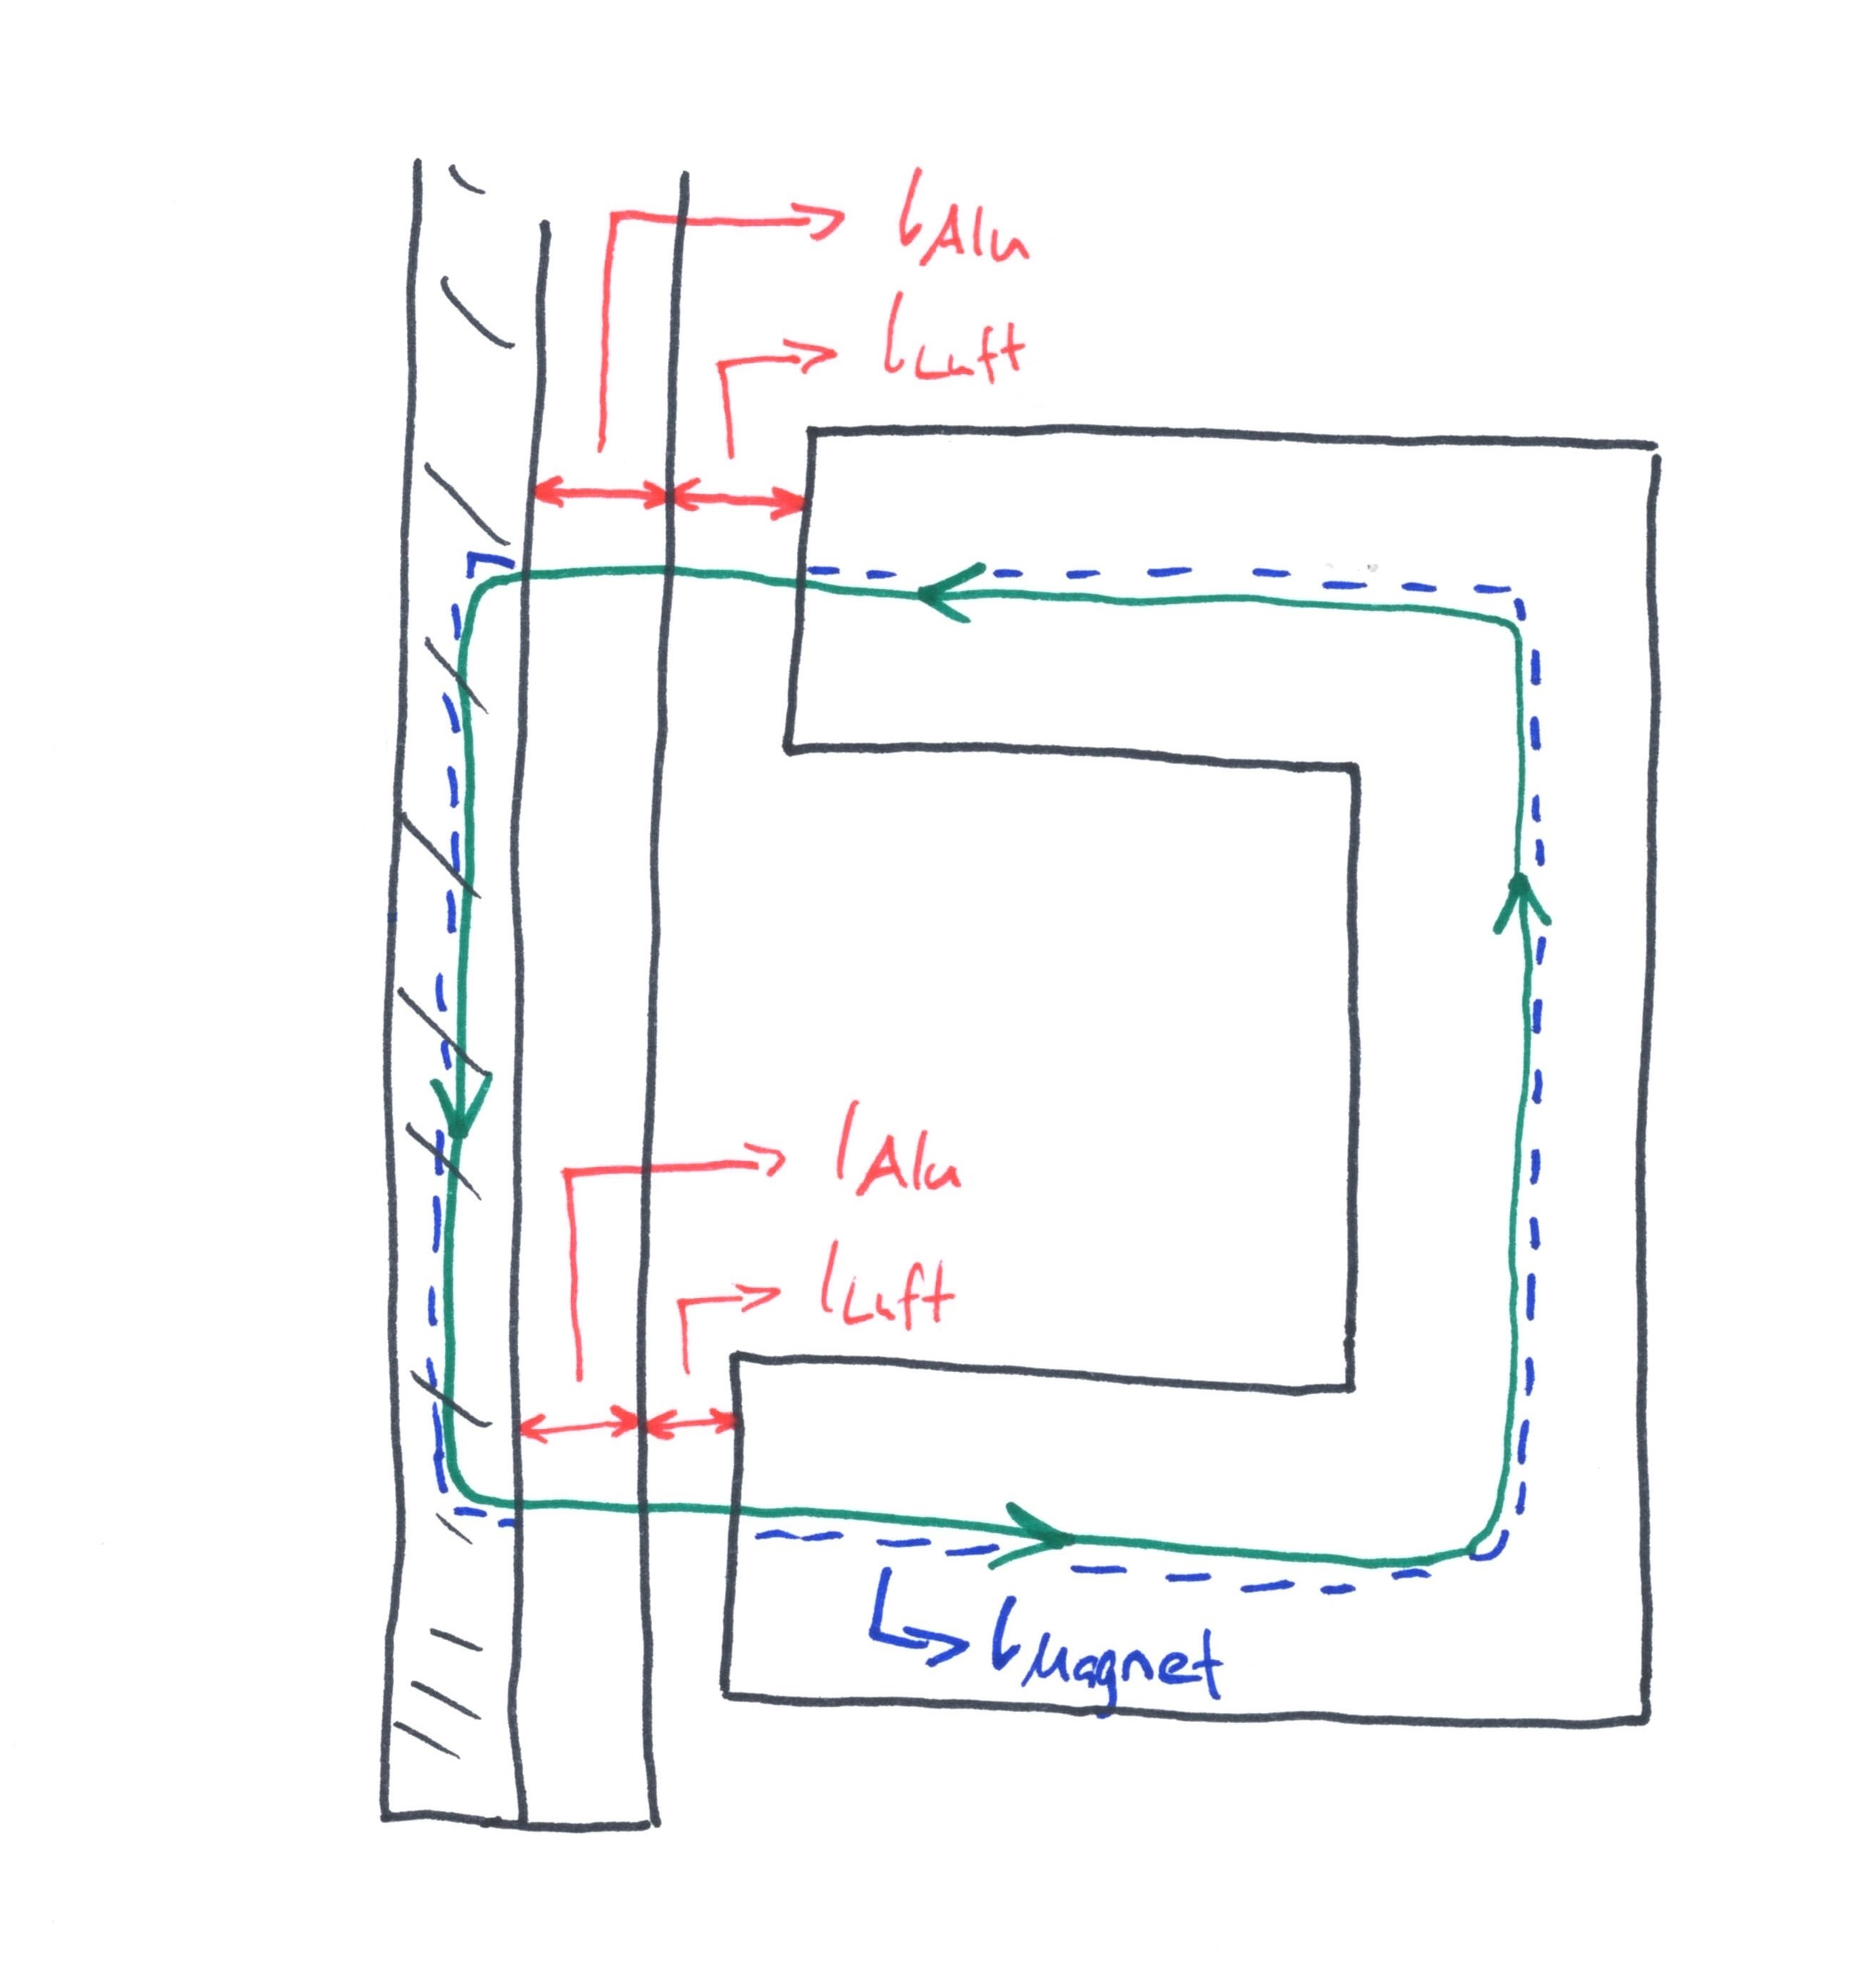
\includegraphics[width=12cm]{assets/images/magnet_design/kreislauf_magnet_corrected}
  \end{center}
  \vspace{-3ex}
  \caption{Magnetkreis bei Magnet und Scheibe}
  \label{fig:magnet_kreisllaenge}
\end{figure}
\newpage
\begin{equation}
  \label{equ:magnetischer_widerstand}
  R_m=\frac{l}{\mu_0 \cdot \mu_r \cdot A}
\end{equation}
\begin{gather}
\shortintertext{\textbf{Begriffe:}}
\begin{tabularx}{0.9\textwidth}{ll}
  $\mu_0$  & magnetische Feldkonstante = 1.257E-06	Vs/Am\\
  $\mu_r$  & Permeabilitätszahl (1 $\equalhat$ Vakuum, $\gg$ 1 $\equalhat$ ferromagnetisch)\\
  $A$	  & Querschnittsfläche des Elements\\
  $R_m$  & Magnetischer Widerstand\\
  $l$	  & Länge des magnetischen Kreises (Siehe Abbildung \ref{fig:magnet_kreisllaenge})
\end{tabularx}\nonumber
\end{gather}
(\cite{schulmaterial_magnetismus})
\newpara
Mit dem magnetischen Widerstand (Siehe Formel \ref{equ:magnetischer_widerstand}) wird in Kombination mit der magnetischen Durchflutung die Magnetstärke (magnetischer Fluss) berechnet. Wird ein starkes Magnet benötigt, wird je nach Möglichkeit entweder die Durchflutung angepasst oder der magnetische Widerstand durch Verkleinerung des Luftspaltes.
\newpara
Der Luftspalt reduziert die magnetische Flussdichte, was den Magneten davon abhält, gesättigt zu werden. Ist ein Magnet gesättigt, wird überflüssige Energie in Wärme umgewandelt. Der Effekt des Luftspalts ist wegen dem magnetischen Widerstand des Vakuums. Die Permeabilitätszahl vom Vakuum ist gleich $1$ und entspricht daher der magnetischen Feldkonstante ($\mu_0 \cdot 1 = \mu_0$). Bereits bei einer Querschnittsfläche von $1m^2$ und einem Luftspalt von $1m$ beträgt der magnetische Widerstand $\frac{1m}{1\cdot 1.257\cdot 10^{-6}\frac{N}{A^2}\cdot 1m^2}=795'798\frac{A}{Vs}$. Bei einem Eisenstück mit einer Permeabilitätszahl von $10'000$ würde der magnetische Widerstand $\frac{1m}{10'000\cdot 1.257\cdot 10^{-6}\frac{N}{A^2}\cdot 1m^2}=79,58\frac{A}{Vs}$ entsprechen, 10'000 kleiner als der Widerstand des Luftspalts. Der Nachteil des Luftspalts ist die Schwächung der Magnetstärke, was zu einer schwächeren Bremse führt.
\newpara
Bei der Wirbelstrombremse ist es wichtig, ein starkes Magnet zu haben. Das bedeutet, dass einen kleinen magnetischen Widerstand benötigt wird.
\newpara

\begin{equation}
  \label{equ:magnetischer_serie_widerstand}
  R_{mGES}=R_{m Luft}+R_{m Alu}+R_{m Magnet}
\end{equation}
\begin{gather}
\shortintertext{\textbf{Begriffe:}}
\begin{tabularx}{0.9\textwidth}{ll}
  $R_{mGES}$  & magnetische Gesamtwiderstand\\
  $R_{m Luft}$  & mag. Widerstand der Luftspalte\\
  $R_{m Alu}$  & mag. Widerstand der Aluminiumscheibe\\
  $R_{m Magnet}$  & mag. Widerstand des Magneten\\
\end{tabularx}\nonumber
\end{gather}
(\cite{schulmaterial_magnetismus})
\newpara
Der gesamte magnetische Widerstand ist abhängig von der Dicke der Aluminiumscheibe, der Dicke des Luftspalts und die magnetischen Kreislänge des Magneten (Siehe Formel \ref{equ:magnetischer_serie_widerstand}). Abbildung \ref{fig:magnet_design_u_magnet_luftspalt} zeigt den Nachteil eines seitlichen Aufbaus im Vergleich eines C-förmigen Magneten (Siehe Abbildung \ref{fig:magnet_design_c_magnet_luftspalt} folgende Seite).  
\begin{figure}[ht]
\begin{center}
  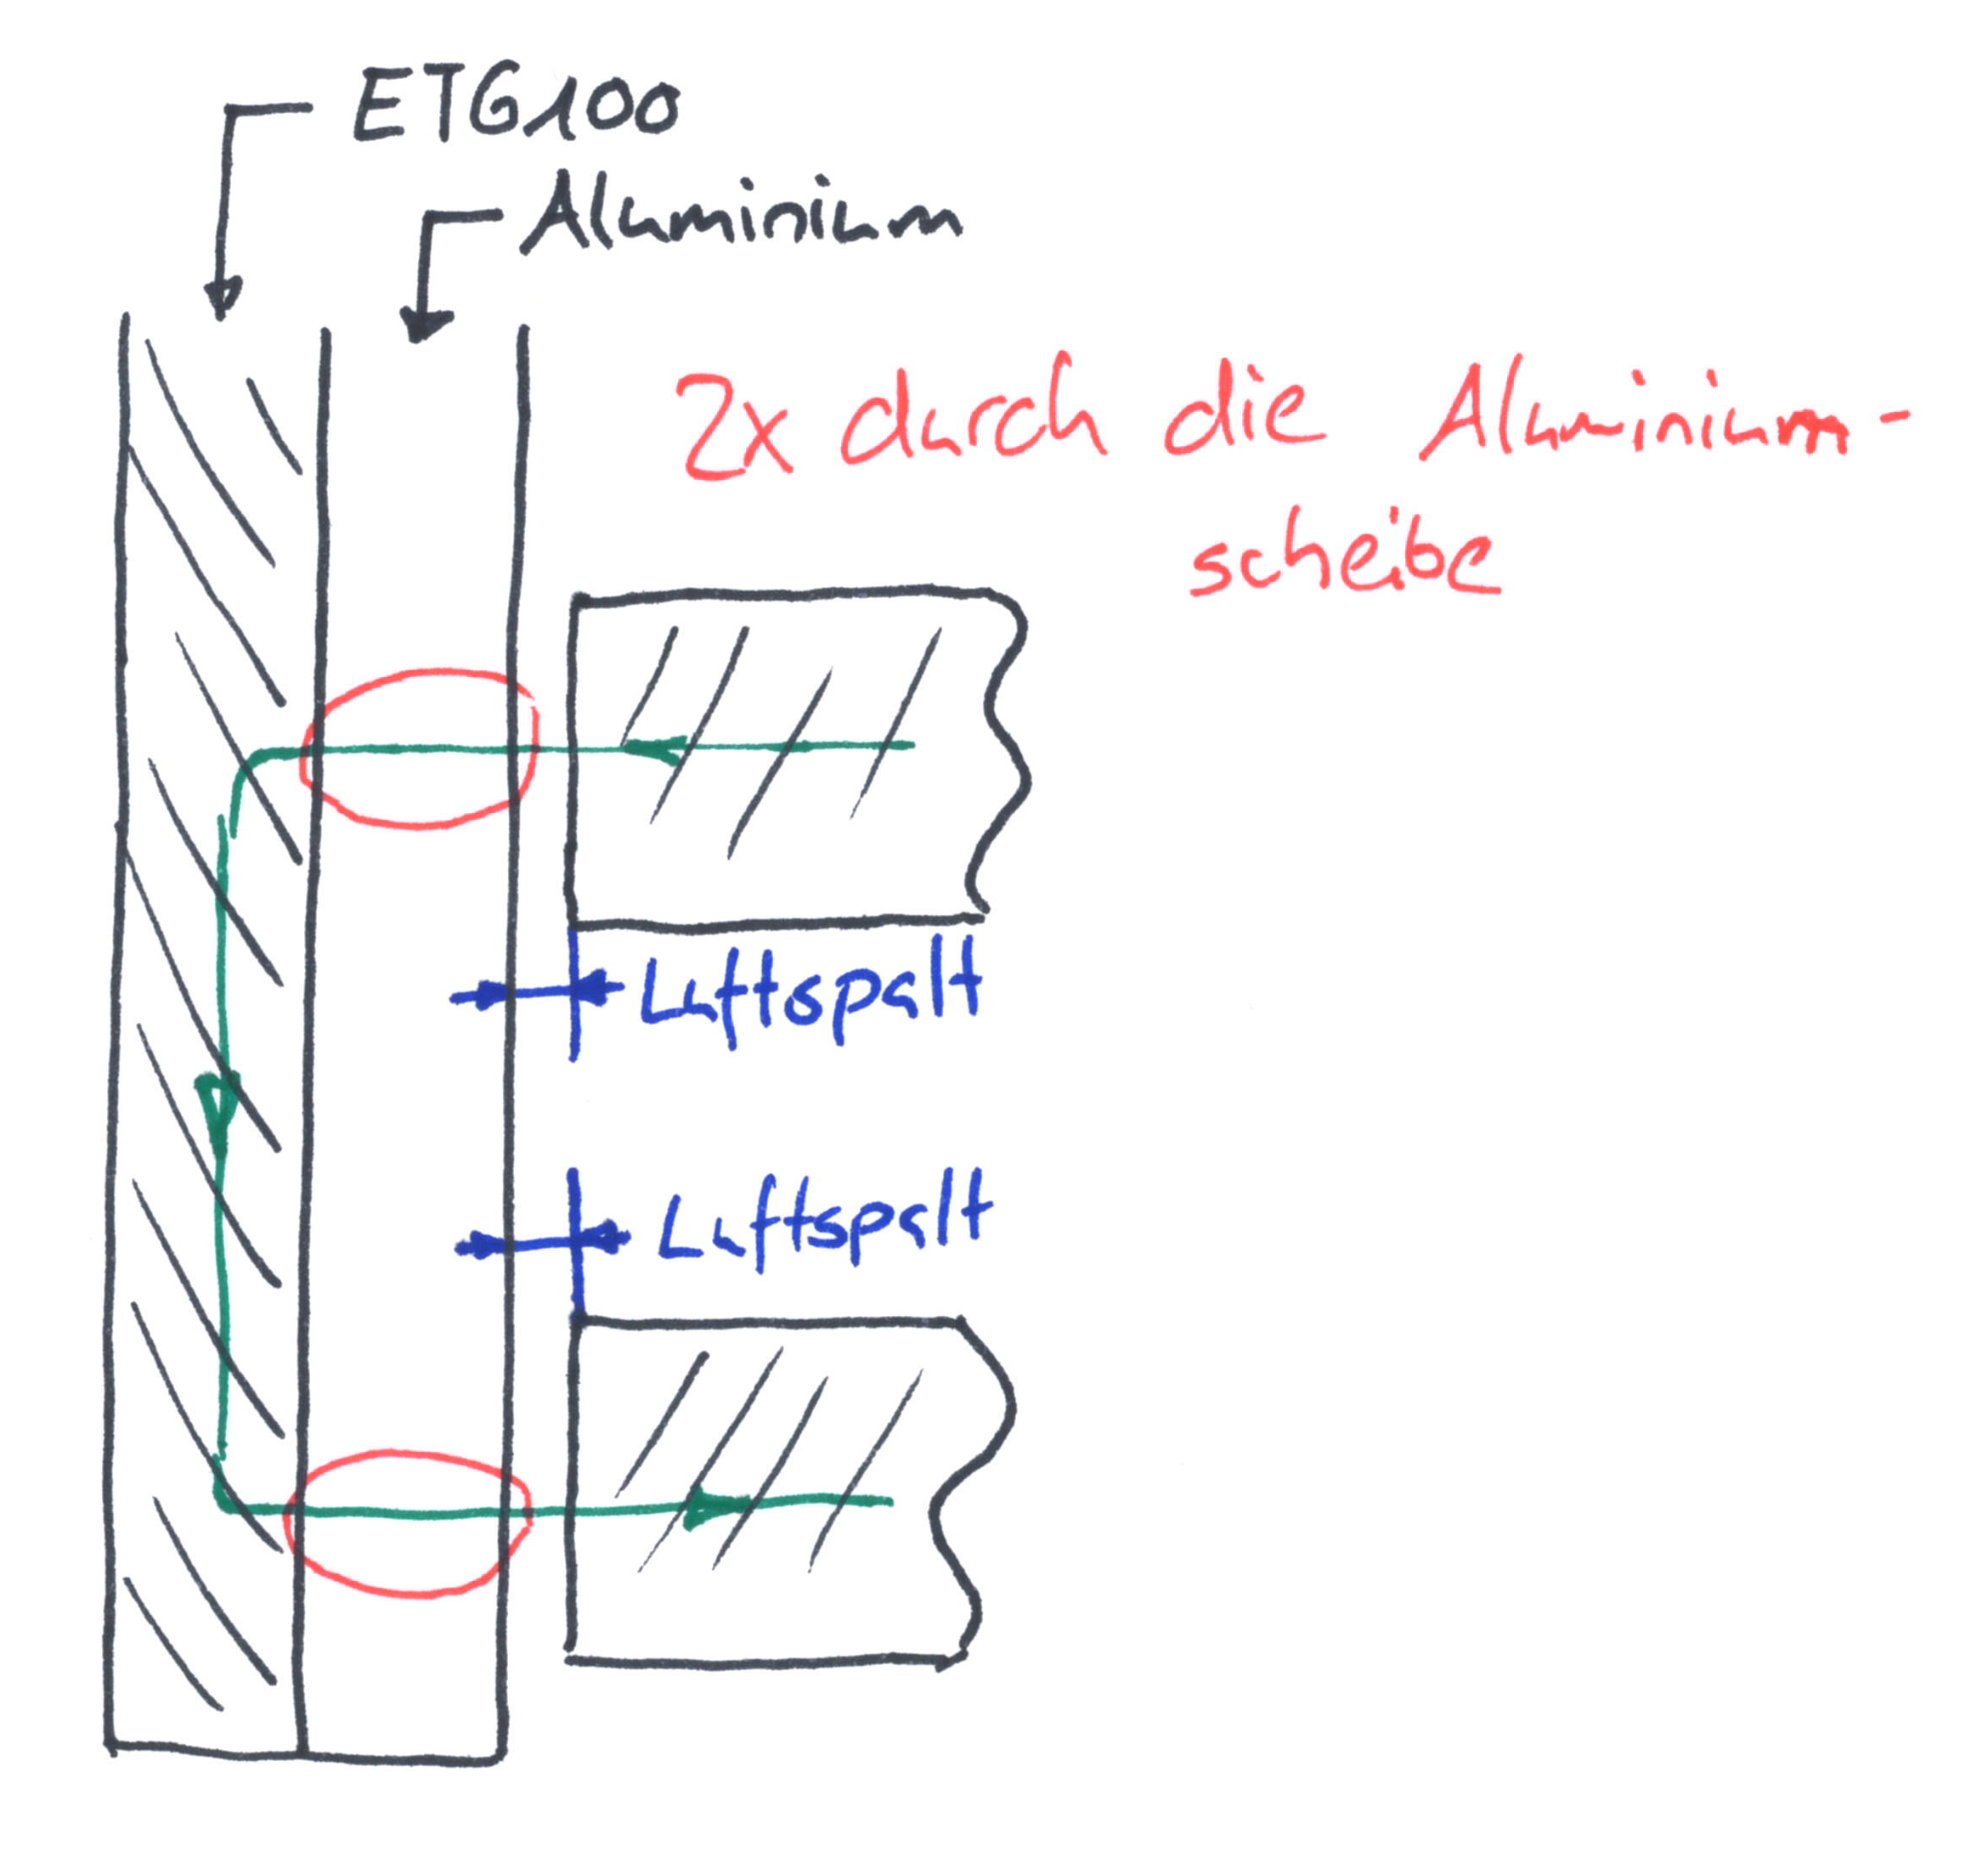
\includegraphics[width=12cm]{assets/images/magnet_design/magnet_luftspalt_u_formig}
\end{center}
\vspace{-3ex}
\caption{Luftspalt eines U-förmigen Magnets}
\label{fig:magnet_design_u_magnet_luftspalt}
\end{figure}

\begin{figure}[ht]
\begin{center}
  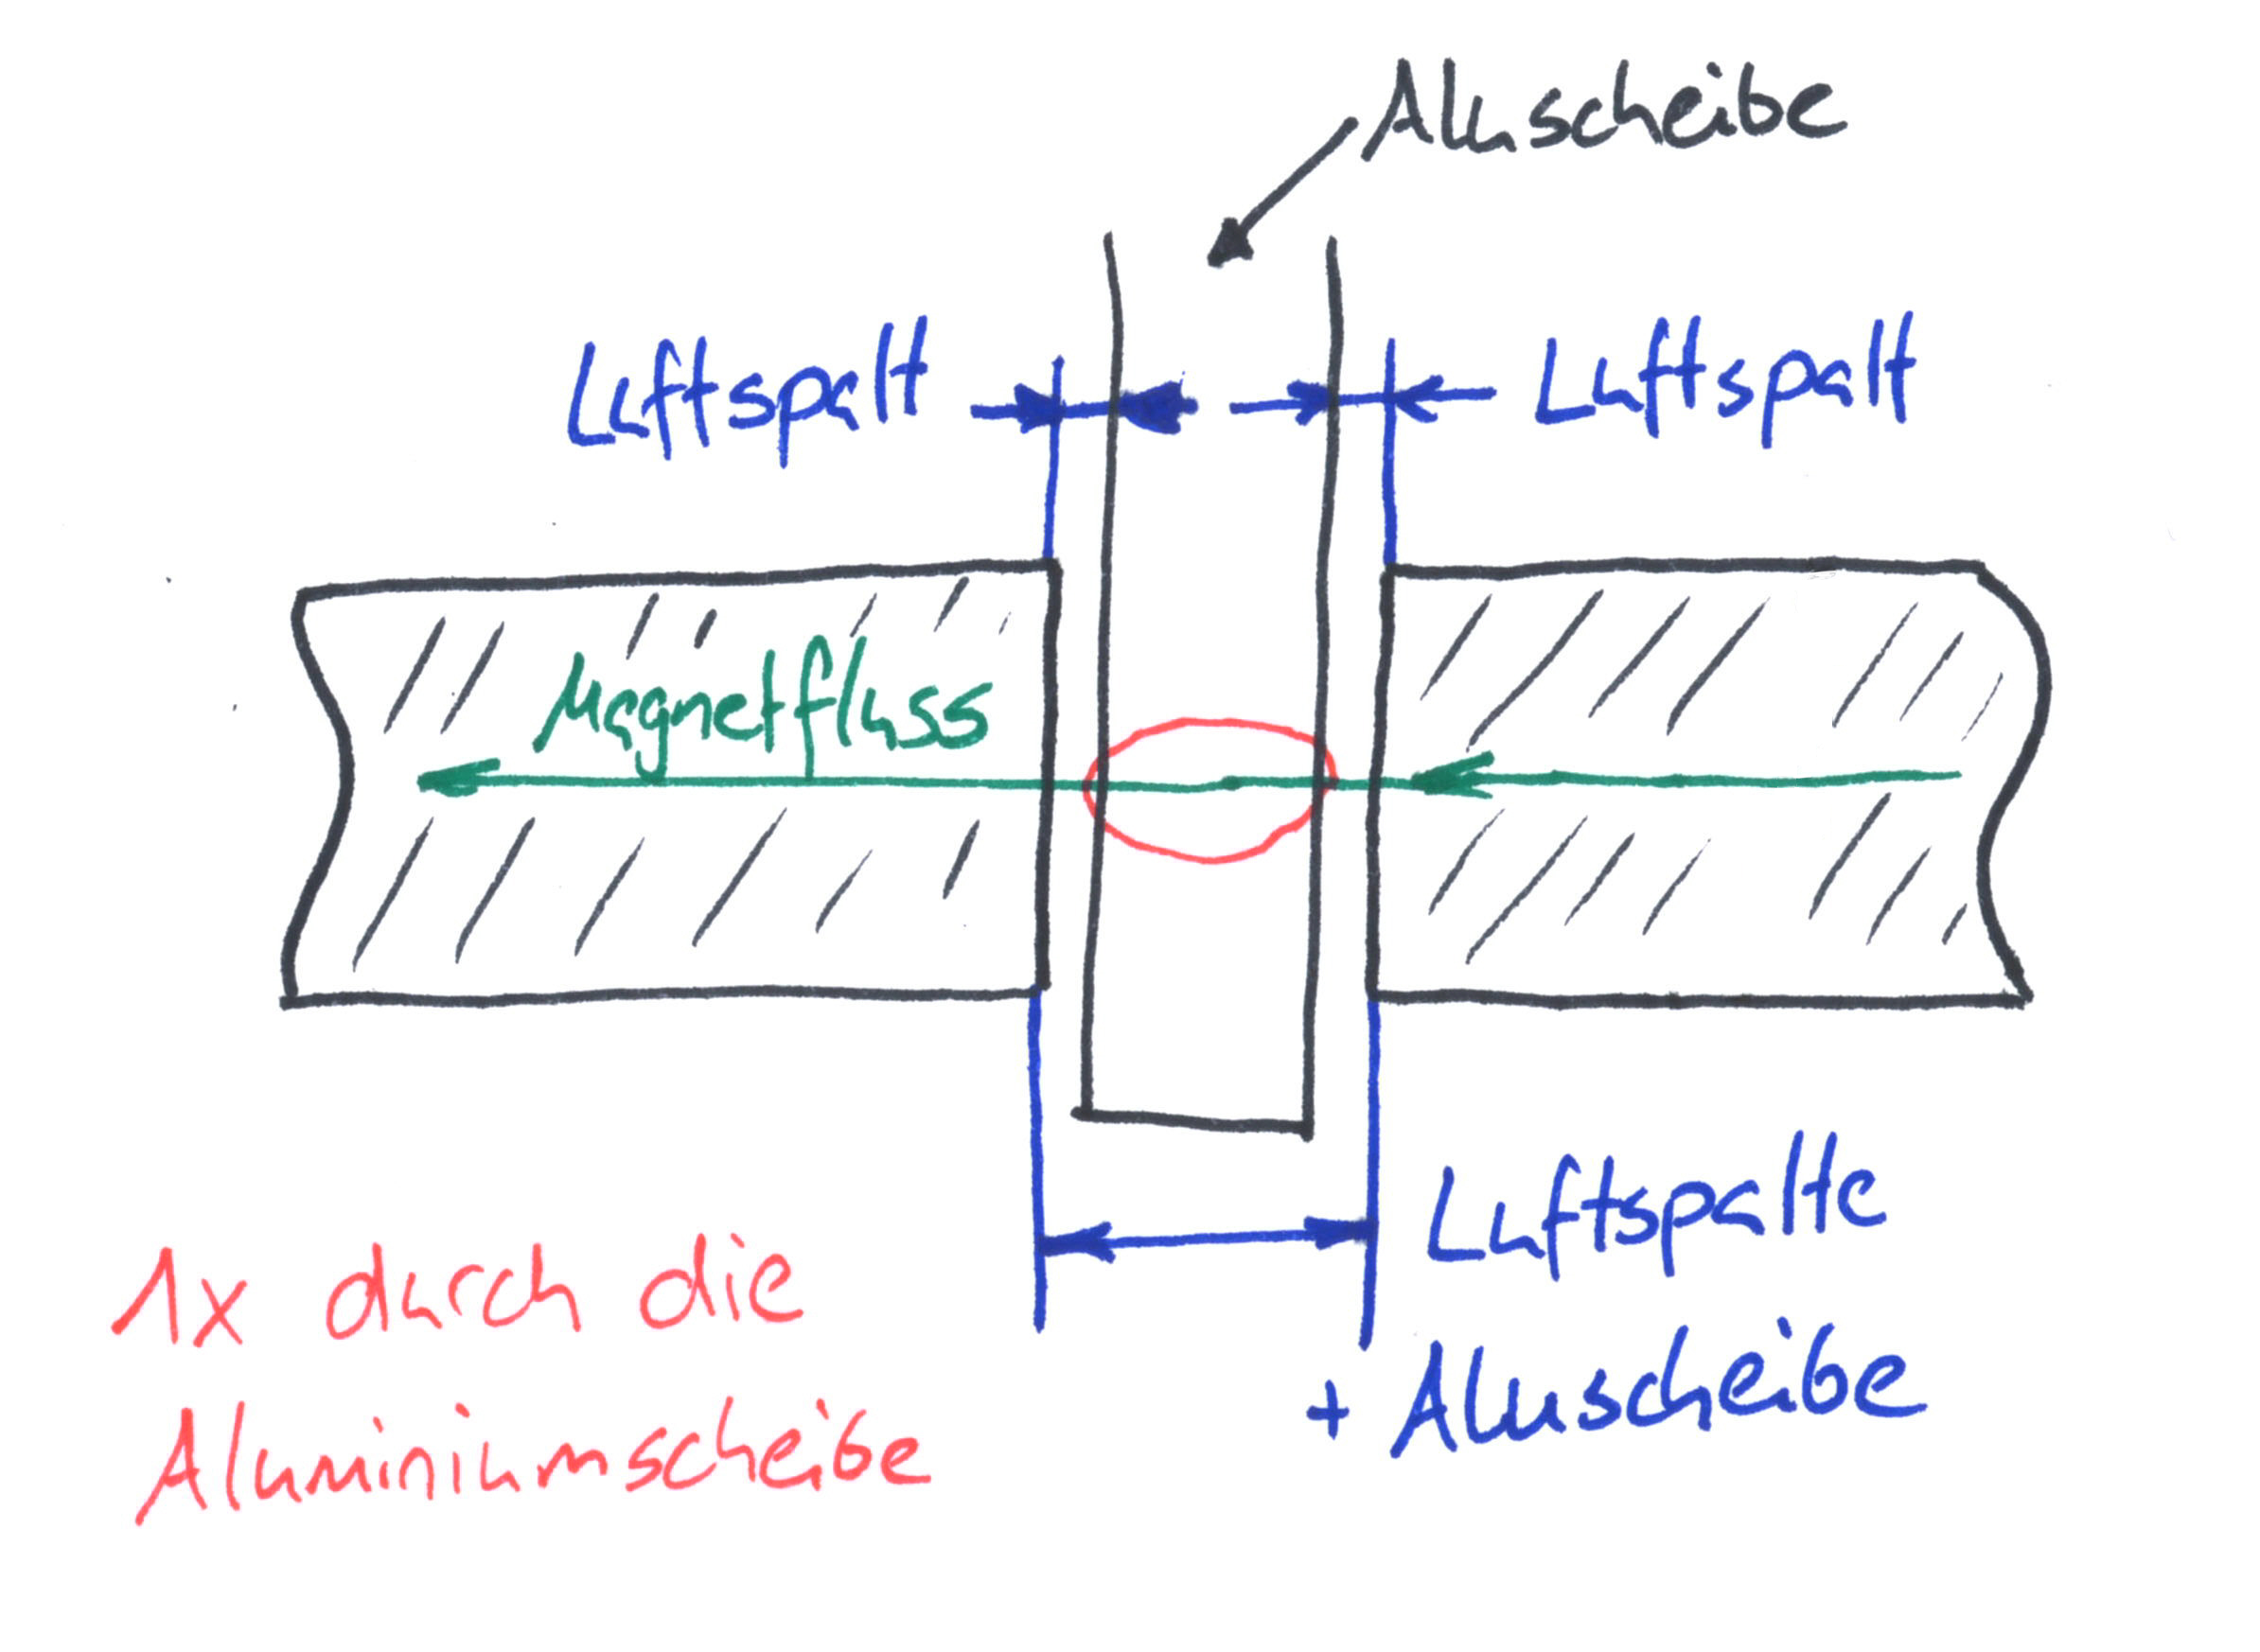
\includegraphics[width=12cm]{assets/images/magnet_design/magnet_luftspalt_c_formig}
\end{center}
\vspace{-3ex}
\caption{Luftspalt eines C-förmigen Magnets}
\label{fig:magnet_design_c_magnet_luftspalt}
\end{figure}

Der Luftspalt kann gleich behalten werden, aber die Kreislänge der Aluminiumscheibe verdoppelt sich, was zu einem doppelten Aluminiumwiderstand führt (Siehe Formel \ref{equ:magnetischer_widerstand_alueinfluss}). Da Aluminium dem Vakuum sehr nahe kommt, hat dies einen grossen Einfluss auf die Magnetstärke.

\begin{equation}
  \label{equ:magnetischer_widerstand_alueinfluss}
  R_m=R_{m Luft}+2 \cdot R_{m Alu}+R_{m Magnet}
\end{equation}
\newpara
Das Drehmoment M in der Formel \ref{equ:smythe_rotation_included} wird durch das Trägheitsdrehmoment ersetzt (Siehe Formel \ref{equ:Drehmoment_tragheit}), da die Bremse abhängig von der zu bremsenden Scheibe ist.

\begin{equation}
  \label{equ:Drehmoment_tragheit}
  M=J\cdot\alpha
\end{equation}
\begin{gather}
\shortintertext{\textbf{Begriffe:}}
\begin{tabularx}{0.9\textwidth}{ll}
  $M$  & Drehmoment\\
  $J$  & Trägheitmoment\\
  $\alpha$ & Winkelbeschleunigung
\end{tabularx}\nonumber
\end{gather}
(\cite[S.127]{kuchling2014taschenbuch})
\newpara
Das Trägheitsmoment gibt die Beeinflussung der Masse von der Scheibe auf die Bremse an (Siehe Formel \ref{equ:tragheitsmoment}). Die Winkelgeschwindigkeit gibt die zeitliche Änderung der Winkelgeschwindigkeit innerhalb von zwei Zeitpunkten an (Siehe Formel \ref{equ:winkelbeschleunigung}).

\begin{equation}
  \label{equ:tragheitsmoment}
  J=m\cdot r^2
\end{equation}
\begin{gather}
\shortintertext{\textbf{Begriffe:}}
\begin{tabularx}{0.9\textwidth}{ll}
  $J$  & Trägheitsmoment\\
  $m$  & Masse der Scheibe\\
  $r$ & Radius der Scheibe
\end{tabularx}\nonumber
\end{gather}
(\cite[S.131]{kuchling2014taschenbuch})
\newpara
\begin{equation}
  \label{equ:winkelbeschleunigung}
  \alpha=\frac{\Delta\omega}{\Delta t}
\end{equation}
\begin{gather}
\shortintertext{\textbf{Begriffe:}}
\begin{tabularx}{0.9\textwidth}{ll}
  $\Delta\omega$  & Kreisfrequenzänderung während der Zeit $\Delta t$\\
  $\Delta t$  & Zeit während zwei Zeitpunkten \\
\end{tabularx}\nonumber
\end{gather}
(\cite[S.88]{kuchling2014taschenbuch})
\newpara
Die Kreisfrequenzänderung und die Zeitdifferenz sind bei der Berechnung Annahmen (der Wert wurde von der Gruppe vorgegeben).
\newpara
Nun wurde die Formel \ref{equ:tragheitsmoment} und die Formel \ref{equ:winkelbeschleunigung} in die Formel \ref{equ:Drehmoment_tragheit} eingesetzt, was zu einer neuen Formel führt (Formel \ref{equ:tragheitsmoment_kombiniert}). Die Dimensionierung basiert nun auf dem \textit{Trial-and-Error} Prinzip. Mit unterschiedlichen Dimensionen wird die Formel (Formel \ref{equ:smythe_rotation_included}) verwendet, bis anhand eines nutzbaren Resultats die Dimensionen des Magnets ermittelt werden konnte. 
\newpara
\begin{equation}
  \label{equ:tragheitsmoment_kombiniert}
  M=\frac{m\cdot r^2\cdot\Delta\omega}{\Delta t}
\end{equation}
\newpara
Folgende Angaben wurde für den aktuellen Magneten verwendet:
\newpara
\begin{tabularx}{0.9\textwidth}{lll}
$\mu_R$	       & $3000$		&Annahme, da kein definitiver Wert existiert\\
$N$	           & $300$		\\
$I$	           & $2 A$\\
$l_{LUFT}$	   & $8 mm$\\
$l_{Fe}$ 	     & $1.05 mm$\\
$a$	           & $0.015 m$\\
$b$	           & $0.003 m$\\
$c$	           & $0.1 m$\\
$A$	           & $0.15 m$\\
$n_{MAX}$	     & $25 s^{-1}$	\\
$\Delta\omega$ & $5 s^{-1}$	  &	Gewünschte Abbremsung innerhalb $\Delta t$\\
$\Delta t$	   & $5 s$        &	Zeit für $\Delta\omega$\\
$\alpha$	     & $1 rad\cdot s^{-2}$&	Winkelbeschleunigung von $\Delta t$ und $\Delta\omega$\\
$m_{RAD}$	     & $5.747 kg$	  & Gewicht des Rades\\
$\Phi$	       & $76.43\cdot 10^{-6} Vs$\\
$\gamma$	     & $6.21\cdot 10^{6} Sm^{-1}$
\end{tabularx}\nonumber
\newpara
daraus ergab sich:
\newpara
\begin{tabularx}{0.9\textwidth}{lll}
  $M_{MAG}$	   & $0.0186 Nm$		& Drehmoment der Bremse\\
  $M_{MASS}$   & $0.00647 Nm$		& Trägheit des Rades\\
\end{tabularx}\nonumber
\newpara
Anhand dieser Resultate sollte der Magnet stärker sein als die Massenträgheit der Scheibe. Was sich aber bei den Messungen herausstellte, stimmte dieser Wert nicht überein mit den Resultaten. Die Begründung, warum diese Resultate nicht stimmen, wird im Kapitel \ref{cap:diskussion} erläutert.
\newpara
\begin{tcolorbox}
  Hier geschahen der erste und zweite Fehler: 1) das Trägheitsdrehmoment (Formel \ref{equ:Drehmoment_tragheit}) wurde nicht mit der Formel von Smythe (Formel \ref{equ:smythe_rotation_included}) kombiniert, sondern die beiden Drehmomente wurden verglichen, was zu einem eher ungenauen Magneten führte. 
  \newpara
  2) Der zweite Fehler ist die Fehlberechnung der Dimensionen. Anstatt die Formel (Formel \ref{equ:smythe_rotation_included}) korrekt zu verwenden wurde stattdessen mit der folgenden Formel (Formel \ref{equ:wrong_calculation}) gerechnet. Die Winkelfrequenz-Formel wurde nicht korrekt eingesetzt und gekürzt, was zu einem falschen Resultat führte.

  \begin{equation}
    \label{equ:wrong_calculation}
    M=\frac{n_{MAX}\cdot b\cdot\gamma\cdot\Phi^2\cdot c^2}{2\cdot\pi\cdot a^2}\cdot(1-\frac{A^{2}\cdot a^{2}}{(A^{2}-c^{2})^{2}})
  \end{equation}
  \newpara
  Im Kapitel \ref{cap:diskussion} wird die vollständige Formel aufgeführt.
\end{tcolorbox}